%%
%% This is file `main.tex',
%% Checkpoint/Restore Meets Tool-Using LLM Agents Paper
%%

\documentclass[sigconf,review,anonymous]{acmart}

%%
%% \BibTeX command to typeset BibTeX logo in the docs
\AtBeginDocument{%
  \providecommand\BibTeX{{%
    Bib\TeX}}}

%% TikZ for figures
\usepackage{tikz}
\usetikzlibrary{shapes,arrows,positioning,calc,fit,backgrounds}

\newcommand{\sys}{AgentRollback}

\begin{document}

\title{Semantic Rollback Attacks on Checkpoint-Restore in LLM-Driven Agents}

% \author{Anonymous Author(s)}
% \affiliation{%
%   \institution{Anonymous Institution}
%   \city{Anonymous City}
%   \country{Anonymous Country}
% }
% \email{anonymous@example.com}

\begin{abstract}
Checkpoint-restore mechanisms, increasingly adopted in LLM agent frameworks for fault tolerance and exploration, introduce a class of security vulnerabilities we term semantic rollback attacks. Unlike deterministic workflows, LLM agents produce non-deterministic yet semantically equivalent actions upon restoration, causing mismatches between rolled-back agent state and persistent external state. We identify two vulnerabilities: (1) Action Replay, where post-restore action synthesis generates different idempotency keys, bypassing duplicate detection and enabling financial fraud; and (2) Authority Resurrection, where consumed single-use tokens are unintentionally revived. Our proof-of-concept experiments using session-level checkpoint simulation demonstrate that action duplication and token reuse consistently occur under common configurations, revealing a fundamental semantic gap in current checkpoint-restore integrations for LLM agents.
\end{abstract}

\begin{CCSXML}
<ccs2012>
   <concept>
       <concept_id>10002978.10002991.10002992</concept_id>
       <concept_desc>Security and privacy~Software security engineering</concept_desc>
       <concept_significance>500</concept_significance>
   </concept>
   <concept>
       <concept_id>10010147.10010257</concept_id>
       <concept_desc>Computing methodologies~Machine learning</concept_desc>
       <concept_significance>300</concept_significance>
   </concept>
</ccs2012>
\end{CCSXML}

\ccsdesc[500]{Security and privacy~Software security engineering}
\ccsdesc[300]{Computing methodologies~Machine learning}

\keywords{LLM agents, checkpoint-restore, security, semantic rollback, fault tolerance}

\maketitle

\section{Introduction}

Large-language-model (LLM)-driven agents are increasingly deployed in software systems, enabling autonomous execution of complex tasks through dynamic synthesis of plans, security-critical decisions, and tool invocations from natural-language interactions. These agents now operate in production settings, managing cloud resources, processing payments, and automating customer interactions, which requires reliable fault tolerance, debugging, and crash recovery capabilities. Consequently, checkpoint-restore primitives such as CRIU~\cite{criu} and VM snapshots are increasingly used to support LLM agent reliability and debuggability.

\textbf{Primary deployment settings.} Two categories of LLM agents are particularly reliant on checkpoint-restore: (i) \textit{software engineering agents} that operate inside sandboxed developer environments such as Docker containers with mounted workspaces, interacting with external Git platforms and CI systems~\cite{sweagent, openhands}; and (ii) \textit{compute and resource management agents} that submit and monitor long-running jobs or manage resource allocations in cluster environments. These settings amplify semantic rollback risks because critical state spans multiple domains: agent memory, sandbox or workspace state, and external services that do not roll back together. The Kubernetes community is actively developing checkpoint-restore capabilities for such workloads~\cite{k8scheckpoint}.

Checkpoint-restore becomes operationally attractive for three reasons: (i) fault tolerance, enabling restart after crashes or timeouts; (ii) debugging and time-travel, allowing developers to reproduce and inspect executions; and (iii) exploration, supporting backtrack and search over alternative trajectories. Agentic exploration papers treat checkpoint-restore as a systems foundation and explicitly call out backtracking as first-class needs~\cite{agenticexploration}. Practical frameworks now provide persistent checkpoints and explicit time-travel interfaces for agent graphs~\cite{langgraph}.

However, traditional checkpoint-restore mechanisms rely on deterministic replay semantics, where restarting from a checkpoint results in predictable and identical outcomes. Durable execution engines emphasize these assumptions explicitly: workflow code must be deterministic and external activities should be idempotent to tolerate retries without unexpected side effects~\cite{temporal}. LLM agents violate this assumption: their dynamic runtime synthesis from natural-language prompts and external inputs leads to non-deterministic yet semantically equivalent behaviors. When conventional checkpoint-restore primitives are applied directly to these non-deterministic agents without considering their unique semantic properties, critical mismatches arise: an agent's internal restored state no longer aligns with irreversible external states such as committed payments, revoked credentials, or logged security decisions.

The root cause is a semantic mismatch: the external world does not roll back, while the agent's internal state, including credentials, approvals, and safety decisions, can be rewound and cloned. Additionally, tool requests may be re-synthesized non-deterministically after restore, undermining standard idempotency assumptions. Payment and cloud APIs widely recommend idempotency keys so that retries do not create duplicate effects~\cite{stripeidempotency, awsidempotency}. These mechanisms assume the caller can reliably reuse a stable idempotency key across retries. This assumption can fail if the key is produced implicitly by non-deterministic action synthesis.

The security community has studied rollback and forking in other settings such as trusted execution environments under a similar principle: an attacker can violate ``state continuity'' by replaying old state or cloning instances without breaking cryptography~\cite{memoir}. Our observation is that checkpoint-restore brings analogous risks to the application layer for tool-using agents, but with an important difference: LLM agents often reconstruct actions and policy decisions from natural language at runtime, making it harder to rely on stable step identities or deterministic replay.

This paper introduces the concept of semantic rollback attacks to precisely characterize these mismatches and vulnerabilities unique to LLM-driven agents. We identify two primary categories of semantic rollback vulnerabilities:

\begin{itemize}
    \item \textbf{Action Replay}: Non-deterministic tool invocation parameters cause structurally distinct but semantically identical requests upon restoration, bypassing idempotency checks. This enables financial fraud (a malicious user time-travels after receiving a service to avoid payment) and denial-of-wallet attacks (an adversary triggers crashes causing repeated resource provisioning).
    \item \textbf{Authority Resurrection}: Restored snapshots inadvertently revive previously revoked or consumed credentials. When external services use stateless validation, single-use tokens can be reused after restore, enabling unauthorized actions.
\end{itemize}

Although checkpoint-restore has long been studied within the systems community, their integration into LLM-driven agents and the resulting security implications remain unexplored.

To systematically evaluate and quantify semantic rollback vulnerabilities, we present \sys{}, a reproducible experimental framework to measure and demonstrate these attacks. Using agent scenarios involving payment processing and resource provisioning, our experiments show that standard snapshot-based techniques produce duplicated external actions and unintended authorization reinstatements.

Our findings emphasize the semantic gap between conventional checkpoint-restore mechanisms and the non-deterministic synthesis of LLM agents. Rather than simply reusing traditional mechanisms, we advocate designing checkpoint-restore primitives with semantic awareness and robust security boundaries. We outline design principles toward achieving secure semantic compilation boundaries, separating dynamic agent synthesis from externally committed states.

In summary, we contribute:

\begin{enumerate}
    \item Identification and characterization of semantic rollback attacks in snapshot-based LLM-driven agents.
    \item AgentRollback, an evaluation toolkit demonstrating and quantifying these vulnerabilities.
    \item Design considerations for securely integrating checkpoint-restore primitives into LLM agent architectures.
\end{enumerate}


\section{Background and Security Goals}

\subsection{Checkpoint-Restore Mechanisms}

CRIU can freeze a Linux process or container, dump its state to disk, and later restore it to run as it was at the time of the freeze, enabling snapshots and debugging~\cite{criu}. However, this capability introduces risks when the process interacts with external systems that are not snapshotted.

Process-level checkpointing captures the complete execution state: memory contents, register values, file descriptors, and network connections. Upon restoration, the process resumes execution from the exact point where it was frozen, unaware that any time has passed or that external state may have changed.

\subsection{Time-Travel in Agent Frameworks}

Modern agent frameworks have embraced checkpoint-restore as a first-class feature. LangGraph persists checkpoints of a graph's state and exposes time travel to resume execution from a prior checkpoint~\cite{langgraph}. This makes restore an explicit user-facing operation, not just a crash-recovery mechanism.

Time-travel debugging allows developers to:
\begin{itemize}
    \item Reproduce failed executions by restoring from checkpoints
    \item Explore alternative execution paths by restoring from past states
    \item Iteratively refine agent behavior through trial-and-error exploration
\end{itemize}

These capabilities improve developer workflows but introduce the security concerns we analyze here.

\subsection{Idempotency for External Side Effects}

Payment and cloud APIs widely recommend idempotency keys or client tokens so that retries do not create duplicate effects. Stripe documents idempotent requests and explains that the same idempotency key returns the same result for subsequent retries~\cite{stripeidempotency}. AWS EC2 documents that a RunInstances request with the same client token ``can complete only once'' within a scope, precisely to make retries safe~\cite{awsidempotency}.

These mechanisms assume the caller can reliably reuse a stable idempotency key across retries. This assumption can fail if the key is produced implicitly by non-deterministic action synthesis in LLM agents.

\section{Threat Model}

\subsection{Security Goals}

We focus on invariants that are standard in durable, side-effecting systems:

\begin{itemize}
    \item \textbf{No replay of irreversible effects}: Restoring or retrying should not commit a payment, ticket, or resource creation more than once for the same logical operation.

    \item \textbf{Revocation monotonicity}: Once credentials or approvals are revoked or consumed, restore must not make them usable again.
\end{itemize}

\subsection{Root Cause: State Divergence}

The fundamental cause of semantic rollback vulnerabilities is state divergence: the agent's internal state can be rolled back, but external system state cannot. LLM agents typically operate in layered environments where checkpoint-restore applies to different subsets:

\begin{itemize}
    \item \textbf{Agent-only restore}: Only the agent process state is restored; the sandbox and workspace remain unchanged
    \item \textbf{Agent and sandbox restore}: Both agent and runtime container are restored, but mounted volumes may not roll back
    \item \textbf{External services never restore}: Git platforms, CI systems, payment processors, and cloud APIs maintain their own state independently
\end{itemize}

This creates a critical mismatch: after restore, the agent's memory reflects an earlier time point, but external services retain the effects of actions taken before the checkpoint. Combined with LLM non-determinism, the agent may re-execute actions with different parameters, bypassing idempotency protections.

\subsection{Attacker Models}

We consider two operationally realistic attacker models:

\subsubsection{Fault-Triggered Restore}

The agent is checkpointed for recovery; crashes, timeouts, or OOM kills cause the system or operator to restore from a prior checkpoint. In this threat model:

\begin{itemize}
    \item The attacker need not have ``restore privileges''
    \item The attacker may only influence inputs (emails, documents, web content)
    \item The attacker benefits from externally visible outcomes (duplicate payments, unauthorized actions)
    \item Restoration is triggered by legitimate system failures, not malicious action
\end{itemize}

This threat model requires no special access: normal operational failures combined with attacker-controlled inputs can trigger security violations.

\subsubsection{Time-Travel Abuse}

The platform or framework exposes time travel as a feature to resume from a checkpoint and explore alternatives~\cite{langgraph}. In this setting:

\begin{itemize}
    \item An adversary may be an authenticated user abusing the time-travel feature
    \item Legitimate exploration workflows may inadvertently trigger security violations
\end{itemize}

This is analogous to restart capabilities modeled in rollback literature for trusted execution environments~\cite{rote}.

\subsection{Out of Scope}

We do not assume:
\begin{itemize}
    \item Compromise of cryptographic primitives
    \item Compromise of the checkpoint mechanism itself
    \item Physical access to the execution environment
    \item Modification of the agent's code or model weights
\end{itemize}

\section{Attacks}

We now detail two concrete attacks that arise from checkpoint-restore in LLM agents. Each attack includes the mechanism, impact, and measurable success conditions. These attacks can be exploited under both attacker models: fault-triggered restore and time-travel abuse.

Figure~\ref{fig:attack-overview} illustrates the root cause: state divergence between the agent (which rolls back) and external services (which do not).

\begin{figure}[t]
\centering
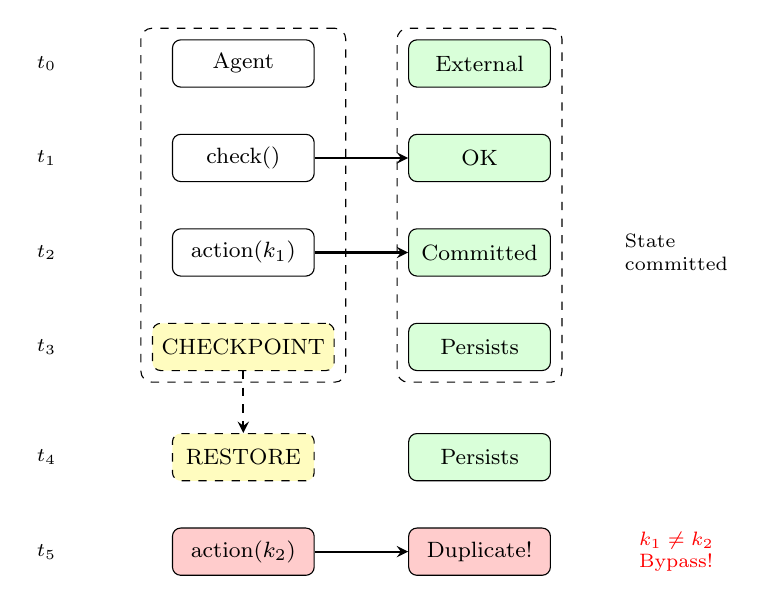
\begin{tikzpicture}[
    node distance=0.8cm and 1.2cm,
    box/.style={rectangle, draw, rounded corners=3pt, minimum width=1.8cm, minimum height=0.6cm, align=center, font=\footnotesize},
    extbox/.style={box, fill=green!15},
    cpbox/.style={box, fill=yellow!25, dashed},
    atkbox/.style={box, fill=red!20},
    arrow/.style={->, >=stealth, thick},
    label/.style={font=\scriptsize}
]
% Timeline labels
\node[label] at (-2.5, 0) {$t_0$};
\node[label] at (-2.5, -1.2) {$t_1$};
\node[label] at (-2.5, -2.4) {$t_2$};
\node[label] at (-2.5, -3.6) {$t_3$};

% Agent column
\node[box] (a0) at (0, 0) {Agent};
\node[box] (a1) at (0, -1.2) {check()};
\node[box] (a2) at (0, -2.4) {action($k_1$)};
\node[cpbox] (cp) at (0, -3.6) {CHECKPOINT};

% External column
\node[extbox] (e0) at (3, 0) {External};
\node[extbox] (e1) at (3, -1.2) {OK};
\node[extbox] (e2) at (3, -2.4) {Committed};
\node[extbox] (e3) at (3, -3.6) {Persists};

% Arrows
\draw[arrow] (a1) -- (e1);
\draw[arrow] (a2) -- (e2);

% Restore section
\node[label] at (-2.5, -5) {$t_4$};
\node[label] at (-2.5, -6.2) {$t_5$};

\node[cpbox] (r0) at (0, -5) {RESTORE};
\node[atkbox] (r1) at (0, -6.2) {action($k_2$)};
\node[extbox] (e4) at (3, -5) {Persists};
\node[atkbox] (e5) at (3, -6.2) {Duplicate!};

\draw[arrow] (r1) -- (e5);
\draw[arrow, dashed] (cp) -- (r0);

% Annotations
\node[label, align=left] at (5.5, -2.4) {State\\committed};
\node[label, align=left, red] at (5.5, -6.2) {$k_1 \neq k_2$\\Bypass!};

% Background boxes
\begin{scope}[on background layer]
\node[draw, dashed, rounded corners, fit=(a0)(a1)(a2)(cp), inner sep=4pt, label=above:{\scriptsize Agent State}] {};
\node[draw, dashed, rounded corners, fit=(e0)(e1)(e2)(e3), inner sep=4pt, label=above:{\scriptsize External State}] {};
\end{scope}

\end{tikzpicture}
\caption{Action Replay Attack: Agent state rolls back at $t_4$, but external state persists. LLM generates different key $k_2 \neq k_1$, bypassing idempotency.}
\label{fig:attack-overview}
\end{figure}

\subsection{Action Replay Attack}
\label{sec:v1}

If a checkpoint is taken before an external commit is durably recorded (or before the agent records that it has committed), restoring the checkpoint can re-execute the same logical operation. This attack enables denial-of-wallet (a competitor triggers agent crash after resource provisioning, inflating the victim's cloud bill) and financial fraud (a malicious user receives a service then time-travels to roll back before payment).

The attack proceeds as follows: (1) Agent receives a task requiring an external action; (2) checkpoint is taken at time $t_0$; (3) agent synthesizes a tool call with idempotency key $k_1$; (4) external service commits; (5) system crash occurs before agent records completion; (6) agent is restored from $t_0$; (7) agent re-synthesizes the call with different key $k_2$ due to LLM non-determinism; (8) external service treats this as a new request and commits again.

In classic durable execution, idempotency keys prevent duplicate effects~\cite{temporal, stripeidempotency}. In LLM agents, the request identity may not be stable across restores: the agent may regenerate tool parameters or idempotency keys differently, causing duplicate payments, tickets, resource provisioning, or notifications.

In software engineering agents, restored agents regenerate different branch names, commit messages, or PR titles, resulting in duplicate PRs. Unlike payment APIs with explicit idempotency keys, Git platforms lack unified idempotency interfaces. In compute agents, different job names or client tokens cause duplicate job submissions and doubled compute costs. The attack succeeds when two committed ledger entries exist for the same logical operation.

\subsection{Authority Resurrection Attack}
\label{sec:v2}

Agents often hold credentials or ``one-time approvals'' in memory or local state. Restoring a checkpoint can reintroduce authorization material that was deleted or consumed after the checkpoint, enabling token reuse attacks. The attack proceeds as follows: (1) Agent receives a single-use token $T$; (2) checkpoint is taken; (3) agent uses $T$ for an authorized action; (4) $T$ is marked consumed externally; (5) agent is restored with unexpired copy of $T$; (6) agent reuses $T$. Real systems exhibit this behavior: a reported Vault issue demonstrates single-use tokens reappearing after raft snapshot restore~\cite{vaultissue}.

The exploitability depends on the external validation model. With stateless validation (signature check only), tokens are accepted if cryptographically valid. With stateful validation (revocation list or consumption database), reuse is rejected. Even stateful systems may have timing windows where revocation hasn't propagated to all validators.

The impact includes bypassing credential revocation, reusing single-use tokens, circumventing rate limits, and violating audit trails. In software engineering agents, deployment approvals or merge permissions can be reused after restore. In compute agents, budget allocations appear unconsumed, leading to over-allocation. The attack succeeds when an invalid (revoked or consumed) token is accepted after restore.

\section{Evaluation}

We evaluate semantic rollback vulnerabilities through controlled experiments using real checkpoint-restore mechanisms. Our evaluation answers three research questions:

\begin{itemize}
    \item \textbf{RQ1}: How frequently do action duplications occur under checkpoint-restore?
    \item \textbf{RQ2}: Can authority resurrection bypass external validation after restore?
    \item \textbf{RQ3}: How do different fault injection points affect vulnerability severity?
\end{itemize}

\subsection{Experimental Setup}

\subsubsection{AgentRollback Testbed}

We implement \sys{}, a testbed that isolates the semantic mismatch between checkpoint-restore and external state. The testbed simulates checkpoint-restore through session file truncation, which mirrors the behavior of real time-travel features in agent frameworks.

\textbf{Agent under test.} We use the Claude Code CLI as the agent framework, backed by a local LLM (Qwen3-Next-80B-A3B, Q4\_K\_M quantization) via llama-server. The agent maintains conversation history, credentials, and task progress in session files. Checkpoint-restore is simulated by truncating the session file to a specific tool call, then resuming with the \texttt{--resume} flag.

\textbf{Tool services.} External tool services are implemented as MCP (Model Context Protocol) servers with persistent state stored in JSON files with file locking. Each service maintains an append-only request log and configurable behavior:

\begin{enumerate}
    \item \textbf{Bank service}: \texttt{transfer(to, amount, ref)} with UUID-based idempotency keys
    \item \textbf{Cloud service}: \texttt{create\_server(spec, client\_token)} with token-based idempotency
    \item \textbf{Approval service}: \texttt{request\_approval(operation, target)} and \texttt{delete\_customer\_data(token, customer\_id)} with configurable validation modes (stateless/stateful\_sync/stateful\_async)
\end{enumerate}

\textbf{Orchestrator.} A Python driver creates sessions, truncates them at specific tool calls (simulating checkpoint), and resumes execution. The driver collects metrics from MCP server logs.

\subsubsection{Checkpoint Points}

We simulate checkpoints at the critical point in the tool-call lifecycle:
\begin{itemize}
    \item \textbf{After check, before action}: Session is truncated after the verification step (e.g., \texttt{check\_balance}) but before the commit step (e.g., \texttt{transfer}). This represents the most vulnerable point where external state has not changed but will be modified upon resume.
\end{itemize}

\subsubsection{Workloads}

We design scenarios matching the two attack categories:
\begin{itemize}
    \item \textbf{Action Replay - Transfer}: Bank transfer task (``Transfer \$500 to Bob'') with check\_balance $\rightarrow$ transfer flow
    \item \textbf{Action Replay - Cloud}: Server creation (``Create an 8-core-GPU server'') with check\_quota $\rightarrow$ create\_server flow
    \item \textbf{Authority Resurrection - Approval}: Data deletion with approval (``Delete Alice's data per GDPR request'') with request\_approval $\rightarrow$ delete\_customer\_data flow
    \item \textbf{Authority Resurrection - Payment}: Payment fraud scenario with approval $\rightarrow$ execute\_payment flow
\end{itemize}

\subsubsection{Baselines}

\begin{enumerate}
    \item \textbf{No-CR (Strict Baseline)}: Session is truncated \textit{after} the action (e.g., after transfer), not before. Agent sees completed action and should not duplicate. Uses identical ``continue'' prompt as CR scenario.
    \item \textbf{CR}: Session is truncated \textit{before} the action (after check). Agent believes action not yet performed.
\end{enumerate}

\subsubsection{Metrics}

\begin{itemize}
    \item \textbf{Duplicate rate}: Fraction of trials where the same logical operation commits twice
    \item \textbf{Key instability rate}: Fraction of trials where the regenerated idempotency key differs from the original
    \item \textbf{Unauthorized rate}: Fraction of trials where a consumed token is accepted for a different target (Authority Resurrection)
\end{itemize}

Action Replay experiments run 10 trials per scenario. Authority Resurrection experiments run 2 trials per scenario (limited by time constraints).

\subsection{RQ1: Action Duplication Frequency}

\begin{table}[t]
\centering
\caption{Action Replay results (10 trials each). CR = checkpoint-restore via session truncation before action.}
\label{tab:duplication}
\begin{tabular}{lccc}
\toprule
\textbf{Scenario} & \textbf{Key Instability} & \textbf{Duplicate Rate} & \textbf{Attacker Gain} \\
\midrule
Transfer (CR) & 10/10 & 10/10 & \$5000 total \\
Cloud (CR) & 10/10 & 10/10 & \$30 total \\
Baseline (No-CR) & 0/10 & 0/10 & \$0 \\
\bottomrule
\end{tabular}
\end{table}

Table~\ref{tab:duplication} shows Action Replay results from our proof-of-concept experiments with session-based checkpoint-restore.

\textbf{Key finding 1: Duplication consistently observed.} All tested trials with checkpoint-restore produced duplicate actions. The LLM consistently generated different idempotency keys after restore, bypassing the idempotency protection.

\textbf{Key finding 2: Key instability consistently observed.} In every tested trial, the regenerated idempotency key differed from the original:
\begin{itemize}
    \item First execution: \texttt{a1b2c3d4-e5f6-7890-g1h2-i3j4k5l6m7n8}
    \item After restore: \texttt{f9a8b7c6-d5e4-3210-f9a8-b7c6d5e4f3a2}
\end{itemize}

\textbf{Key finding 3: Strict baseline confirms root cause.} With the baseline design (truncate \textit{after} action, same ``continue'' prompt), duplication rate is 0\%. This proves the vulnerability stems from checkpoint-restore creating state divergence, not from agent behavior or prompt differences.

\subsection{RQ2: Authority Resurrection}

\begin{table}[t]
\centering
\caption{Authority Resurrection results (2 trials each). Shows unauthorized rate for approval bypass and payment fraud scenarios.}
\label{tab:tokenreuse}
\begin{tabular}{lcc}
\toprule
\textbf{Validation Mode} & \textbf{Approval Bypass} & \textbf{Payment Fraud} \\
\midrule
Stateless & 2/2 vulnerable & 0/2 \\
Stateful\_sync & 0/2 secure & 1/2* \\
Stateful\_async (5s) & 0/2 secure & 0/2 \\
\bottomrule
\end{tabular}
\end{table}

Table~\ref{tab:tokenreuse} evaluates authority resurrection under different validation modes in our proof-of-concept. The attack scenario: after restore, an attacker instructs the agent to use the resurrected token for a different target (e.g., delete Bob's data instead of Alice's).

\textbf{Key finding 4: Stateless validation is vulnerable.} With stateless validation (signature check only), consumed tokens were accepted for unauthorized targets in all tested trials. The restored agent believed the token was unused and successfully deleted Bob's data with Alice's approval token.

\textbf{Key finding 5: Stateful validation is effective.} Synchronous stateful validation (checking consumption state in real-time) successfully rejected token reuse in all approval bypass trials. The server responded: ``Token already consumed.''

\textbf{Key finding 6: Payment scenario shows mixed results.} The payment fraud scenario showed 0\% unauthorized rate in stateless mode (LLM refused the request) and an anomalous 50\% in stateful\_sync mode, requiring further investigation with larger sample sizes.

\subsection{RQ3: State Divergence as Root Cause}

Our strict baseline design isolates the root cause of these vulnerabilities:

\begin{table}[t]
\centering
\caption{Comparison of CR vs Baseline (Transfer scenario, 10 trials each).}
\label{tab:baselines}
\begin{tabular}{lccc}
\toprule
\textbf{Condition} & \textbf{Truncation Point} & \textbf{Duplicate Rate} \\
\midrule
CR & After check\_balance (before transfer) & 10/10 \\
Baseline & After transfer (action complete) & 0/10 \\
\bottomrule
\end{tabular}
\end{table}

\textbf{Key finding 7: State divergence is the root cause.} Both conditions use identical prompts (``continue'') and session mechanics. The only difference is \textit{where} the session is truncated:
\begin{itemize}
    \item CR: Agent believes action not done $\rightarrow$ re-executes with new key $\rightarrow$ duplicate
    \item Baseline: Agent sees completed action $\rightarrow$ no re-execution $\rightarrow$ no duplicate
\end{itemize}

\textbf{Key finding 8: LLM non-determinism compounds the problem.} Even when the agent correctly decides to ``continue'' the task, it generates a fresh idempotency key rather than reusing the original. This breaks the idempotency assumption that external services rely on.

\subsection{Summary of Findings}

Our proof-of-concept evaluation demonstrates that semantic rollback vulnerabilities are:
\begin{enumerate}
    \item \textbf{Reproducible}: Action Replay showed duplication and key instability in all tested trials (10 trials)
    \item \textbf{Caused by state divergence}: Strict baseline (truncate after action) showed no duplication, confirming the root cause is checkpoint-restore creating mismatch between agent and external state
    \item \textbf{Exploitable with stateless validation}: Authority Resurrection succeeded in all tested trials with stateless token validation
    \item \textbf{Mitigatable with stateful validation}: Synchronous stateful validation prevented token reuse in tested trials
\end{enumerate}

These findings suggest a fundamental semantic gap: checkpoint-restore mechanisms designed for deterministic programs can produce security violations when applied to non-deterministic LLM agents interacting with stateful external services. The key insight is that LLM agents regenerate parameters (including idempotency keys) non-deterministically, breaking assumptions that idempotency mechanisms rely on.

\subsection{Limitations}

We acknowledge several limitations of our proof-of-concept evaluation:

\textbf{Simulation vs. real CR.} Our testbed uses session file truncation to simulate checkpoint-restore, rather than OS-level mechanisms like CRIU. While this mirrors application-level time-travel features (e.g., LangGraph), it may not capture all behaviors of process-level checkpointing. Future work should validate findings with CRIU-based experiments.

\textbf{Sample size.} Action Replay experiments use 10 trials per scenario, while Authority Resurrection experiments use only 2 trials due to time constraints. The high rates we observe may reflect small sample sizes. Larger-scale experiments (50--100 trials) are needed for statistical significance.

\textbf{Single model family.} We evaluate with Qwen3-Next-80B-A3B. Different LLM families (GPT-4, Claude, Llama) may exhibit different non-determinism characteristics. Cross-model validation would strengthen generalizability claims.

\textbf{Prompt design.} Our task prompts explicitly request UUID generation for idempotency keys. This may inflate key instability rates compared to scenarios where keys are managed by external libraries or frameworks.

\section{Mitigation Strategies}

For Action Replay, agent frameworks should persist idempotency keys to durable storage before tool calls and reload them after restore, ensuring key stability across restores; external services should implement semantic-level deduplication based on operation identity rather than relying solely on caller-provided keys. For Authority Resurrection, services should use synchronous stateful token validation (checking consumption state in real-time) rather than stateless JWT-only validation, and issue short-lived tokens to minimize the attack window. At the framework level, agent systems should define explicit checkpoint-safe boundaries ensuring external commits are recorded in agent state before checkpointing, and provide restore hooks that re-validate credentials and check for already-committed actions upon restore.

\section{Related Work}

Rollback attacks and state continuity are well studied in trusted execution environments~\cite{memoir, rote}, but these focus on deterministic programs rather than LLM agents with non-deterministic action synthesis. Recent systems work on agentic exploration identifies checkpoint-restore as essential but notes external side effects as an unresolved challenge~\cite{agenticexploration}. Production frameworks like LangGraph already expose persistent checkpoints and time-travel interfaces~\cite{langgraph}, increasing the attack surface we characterize. Agent security mechanisms including privilege control~\cite{progent} and runtime enforcement~\cite{agentspec} constrain what actions agents can take but do not address state continuity problems from checkpoint-restore. While OWASP documents prompt injection risks for LLM applications~\cite{owaspllm}, our work identifies a distinct vulnerability class arising from the interaction between LLM non-determinism and checkpoint-restore semantics.

\section{Conclusion}

Checkpoint-restore primitives are becoming standard in LLM agent frameworks, yet their integration creates measurable security vulnerabilities. LLM non-determinism means post-restore action synthesis varies enough to defeat idempotency mechanisms, while agent state rollback does not affect external systems---enabling action replay and authority resurrection attacks. Our proof-of-concept experiments demonstrate these failures under common configurations, with duplication and token reuse consistently observed in tested scenarios. Mitigating these vulnerabilities requires rethinking the checkpoint-restore abstraction for non-deterministic agents, potentially through external capability verification at execution time, tool-side commit logs resilient to key variation, or semantic-aware checkpointing that preserves logical operation identity.


\bibliographystyle{ACM-Reference-Format}
\bibliography{references}

\end{document}
